%!LW recipe=latexmk (xelatex)
%!TEX program = xelatex

\documentclass[10pt]{report}

\input{../src/glass/aircraftdata/style.tex}

\runningtitle{Ground Unit Data}
\setcounter{secnumdepth}{0} 
\setcounter{tocdepth}{1} 

\newcommand{\groundunittype}[1]{\subsection{#1}}

\begin{document}

\title{Air Power Ground Unit Data}
\author{Alan Watson Forster}
\date{19 September 2025}

\maketitle
\twocolumn[\section{Ground-Combat Units}]

Ground-combat units represent infantry, tanks and other AFVs, trucks, and artillery. Their primary role is combat with other ground units.

\paragraph{Properties.}

Table \ref{table:ground-combat-units} summarizes the properties of the ground-combat units. Soft and hard defense strengths are suffixed with S and H, respectively. The sighting range is given in hexes. The AAA class is B2 for infantry platoons and B3 for AFV platoons, indicating that they are capable of barrage fire to altitudes of 2 and 3 levels, respectively. VPs are given for K, 2D, and D damage.

\paragraph{Representation.}

Figure \ref{figure:ground-combat-units} shows the graphical representation of the ground-combat units. The representation mainly uses NATO symbols, with some simplifications and two extensions. The first extension is that  a rectangle denotes trucks and other mobile units, just as the armor symbol denotes armored units. The second is that a partial infantry symbol denotes the association of IFVs and APCs with infantry. Also, the designator for heavy, medium, and light armor is placed within rather than below the armor symbol.

\paragraph{Echelon.}

Most units are platoons although some are teams.

\paragraph{Protection.}

Units equipped AFVs are classified as \emph{heavy}, \emph{medium}, or \emph{light} according to their degree of protection. Units equipped with unprotected or incompletely protected vehicles are referred to as being \emph{mobile}.

\paragraph{Mobility.} Wheeled, half-tracked, and tracked vehicles are not distinguished. Thus, armored cars are treated as light tanks (e.g., the AMX-10 RC and Panhard EBR), unarmored tracked cargo-carriers are treated as trucks (e.g., the M548), and incompletely protected artillery with either wheels or tracks are treated as mobile artillery (e.g., the wheeled CAESAR and the tracked M107).


\begin{table*}
    \caption{Ground-Combat Units}
    \centering
    \footnotesize
    \begin{tabular}{lcccccc}
\toprule

            Type&
            \vertical{Echelon}&
            \vertical{\begin{tabular}{@{}l@{}}Defense\\Strength\end{tabular}}&
            \vertical{\begin{tabular}{@{}l@{}}Sighting\\Range\end{tabular}}&
            \vertical{Mobility}&
            \vertical{\begin{tabular}{@{}l@{}}VPs\\3D/2D/D\end{tabular}}&
            \vertical{\begin{tabular}{@{}l@{}}AAA\\Class\tablenotemark{1}\end{tabular}}
            \\
        
\midrule
\addlinespace
Infantry &\wbox[l]{Section}{Platoon}&\wbox[l]{0}{4}&\wbox{00}{6}&U&\wbox{00/00/0}{5/3/2}&B2\\
Infantry HQ &\wbox[l]{Section}{Platoon}&\wbox[l]{0}{4}&\wbox{00}{6}&U&\wbox{00/00/0}{11/7/4}&B2\\
\addlinespace
Infantry FAC &\wbox[l]{Section}{Section}&\wbox[l]{0}{5}&\wbox{00}{6}&U&\wbox{00/00/0}{\wbox[c]{0}{--}/8/4}&---\\
Infantry FAC &\wbox[l]{Section}{Squad}&\wbox[l]{0}{5}&\wbox{00}{6}&U&\wbox{00/00/0}{\wbox[c]{0}{--}/\wbox[c]{0}{--}/4}&---\\
\addlinespace
Heavy Tank &\wbox[l]{Section}{Platoon}&\wbox[l]{0}{\underline{8}}&\wbox{00}{12}&G&\wbox{00/00/0}{12/8/4}&B3\\
Heavy Tank HQ &\wbox[l]{Section}{Platoon}&\wbox[l]{0}{\underline{8}}&\wbox{00}{12}&G&\wbox{00/00/0}{18/12/6}&B3\\
Medium Tank &\wbox[l]{Section}{Platoon}&\wbox[l]{0}{\underline{6}}&\wbox{00}{12}&G&\wbox{00/00/0}{10/7/3}&B3\\
Medium Tank HQ &\wbox[l]{Section}{Platoon}&\wbox[l]{0}{\underline{6}}&\wbox{00}{12}&G&\wbox{00/00/0}{16/11/5}&B3\\
Light Tank &\wbox[l]{Section}{Platoon}&\wbox[l]{0}{\underline{4}}&\wbox{00}{12}&G&\wbox{00/00/0}{6/4/2}&B3\\
Light Tank HQ &\wbox[l]{Section}{Platoon}&\wbox[l]{0}{\underline{4}}&\wbox{00}{12}&G&\wbox{00/00/0}{12/8/4}&B3\\
Open Tank &\wbox[l]{Section}{Platoon}&\wbox[l]{0}{\underline{4}!}&\wbox{00}{12}&G&\wbox{00/00/0}{5/3/2}&B3\\
Open Tank HQ &\wbox[l]{Section}{Platoon}&\wbox[l]{0}{\underline{4}!}&\wbox{00}{12}&G&\wbox{00/00/0}{11/7/4}&B3\\
\addlinespace
Light Anti-Tank &\wbox[l]{Section}{Platoon}&\wbox[l]{0}{\underline{4}}&\wbox{00}{12}&G&\wbox{00/00/0}{10/7/3}&B3\\
\addlinespace
Medium IFV &\wbox[l]{Section}{Platoon}&\wbox[l]{0}{\underline{6}}&\wbox{00}{12}&G&\wbox{00/00/0}{10/6/4}&B3\\
Light IFV &\wbox[l]{Section}{Platoon}&\wbox[l]{0}{\underline{4}}&\wbox{00}{12}&G&\wbox{00/00/0}{6/4/2}&B3\\
\addlinespace
Heavy APC &\wbox[l]{Section}{Platoon}&\wbox[l]{0}{\underline{8}}&\wbox{00}{12}&G&\wbox{00/00/0}{10/7/3}&B3\\
Medium APC &\wbox[l]{Section}{Platoon}&\wbox[l]{0}{\underline{6}}&\wbox{00}{12}&G&\wbox{00/00/0}{8/5/3}&B3\\
Light APC &\wbox[l]{Section}{Platoon}&\wbox[l]{0}{\underline{4}}&\wbox{00}{12}&G&\wbox{00/00/0}{6/4/2}&B3\\
Open APC &\wbox[l]{Section}{Platoon}&\wbox[l]{0}{\underline{4}!}&\wbox{00}{12}&G&\wbox{00/00/0}{5/3/2}&B3\\
\addlinespace
Truck &\wbox[l]{Section}{Platoon}&\wbox[l]{0}{2}&\wbox{00}{12}&P&\wbox{00/00/0}{4/3/1}&---\\
Truck &\wbox[l]{Section}{Section}&\wbox[l]{0}{2}&\wbox{00}{12}&P&\wbox{00/00/0}{\wbox[c]{0}{--}/3/1}&---\\
Truck &\wbox[l]{Section}{Squad}&\wbox[l]{0}{2}&\wbox{00}{12}&P&\wbox{00/00/0}{\wbox[c]{0}{--}/\wbox[c]{0}{--}/1}&---\\
Tracked Carrier &\wbox[l]{Section}{Platoon}&\wbox[l]{0}{2}&\wbox{00}{12}&G&\wbox{00/00/0}{4/3/1}&---\\
\addlinespace
Armored Artillery &\wbox[l]{Section}{Battery}&\wbox[l]{0}{\underline{4}}&\wbox{00}{12}&G&\wbox{00/00/0}{12/8/4}&B3\\
Tracked Artillery &\wbox[l]{Section}{Battery}&\wbox[l]{0}{2}&\wbox{00}{12}&G&\wbox{00/00/0}{10/7/3}&---\\
Mobile Artillery &\wbox[l]{Section}{Battery}&\wbox[l]{0}{2}&\wbox{00}{12}&P&\wbox{00/00/0}{9/6/3}&---\\
Towed Artillery &\wbox[l]{Section}{Battery}&\wbox[l]{0}{4}&\wbox{00}{18}&P&\wbox{00/00/0}{8/5/3}&---\\
\addlinespace
Armored Rocket Artillery &\wbox[l]{Section}{Battery}&\wbox[l]{0}{\underline{4}}&\wbox{00}{12}&G&\wbox{00/00/0}{12/8/4}&B3\\
Mobile Rocket Artillery &\wbox[l]{Section}{Battery}&\wbox[l]{0}{2}&\wbox{00}{12}&P&\wbox{00/00/0}{9/6/3}&---\\
\addlinespace
Tracked Missile Artillery &\wbox[l]{Section}{Battery}&\wbox[l]{0}{2}&\wbox{00}{12}&G&\wbox{00/00/0}{10/7/3}&---\\
Mobile Missile Artillery &\wbox[l]{Section}{Battery}&\wbox[l]{0}{2}&\wbox{00}{12}&P&\wbox{00/00/0}{9/6/3}&---\\
\addlinespace
\bottomrule
\end{tabular}

    \label{table:ground-combat-units}
\end{table*}

\begin{figure*}
    \centering
    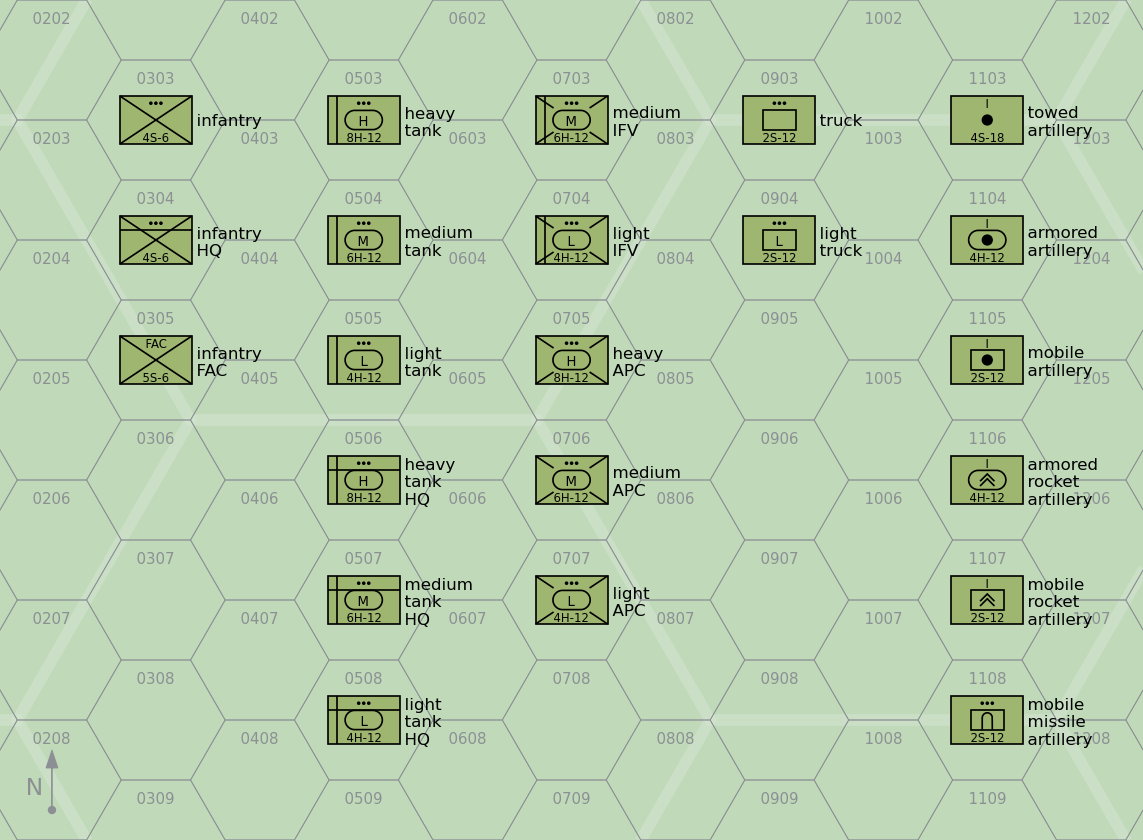
\includegraphics[height=0.4\linewidth]{figure-ground-combat-units.png}
    \caption{Ground-Combat Units}
    \label{figure:ground-combat-units}
\end{figure*}

\paragraph{Infantry.}

Infantry are soldiers trained to fight on foot. The infantry and the infantry HQ units are platoons. The infantry FAC unit is a forward air controller team.

\paragraph{Mechanized and Motorized Infantry.}

A mechanized infantry platoon will be associated with a platoon of APCs or IFVs. A motorized infantry platoon will be associated with a platoon of trucks.

\paragraph{Tanks.}

Tanks are AFVs that are specialized for direct fire. All tank units are platoons. Examples:

\begin{itemize}

    \item Heavy: Conqueror, Chieftain, Challenger 1/2, IS-3, Leclerc, Leopard 2, M1, Merkava, T-10, T-64, T-72, T-80, T-84, and T-90.

    \item Medium: AMX-30, Centurion, Leopard 1, M4 Sherman, M47/48, M60, M103, T-34, T-54/55, and T-62.

    \item Light: AMX-10 RC, AMX-13, Ferret, M24, M41, M551, Panhard EBR, PT-76, and Scorpion/Scimitar.

\end{itemize}

\paragraph{IFVs.}

IFVs are AFVs that carry infantry and provide fire support. They are distinguished from APCs by having a 20 mm or larger cannon. All IFV units are platoons. Examples:

\begin{itemize}

    \item Heavy: none.

    \item Medium: CV90, M2A2 (only), and Marder.

    \item Light: all others including the AMX-10P, BMP-1/2/3, LAV-25, M2/3 (except M2A2), M1296, VCBI, and Warrior.

\end{itemize}

\paragraph{APCs.}

APCs are AFVs that carry infantry but do not provide significant fire support. All APC units are platoons. Heavy and medium APCs are typically converted tanks. Examples:

\begin{itemize}

    \item Heavy: converted heavy tanks.

    \item Medium APCs: converted medium tanks.

    \item Light APCs: all others, including the BTR-152, BTR-40, BTR-50/60/70/80, FV432, M3 half-track, M113, M114, Saracen, Spartan, most Stryker variants, and VAB.

\end{itemize}

\paragraph{Trucks.}

Trucks are unarmored or incompletely armored vehicles. All truck units are platoons.

Light trucks include Humvees, Jeeps, and Land Rovers.

\paragraph{Artillery.}

Artillery is specialized for indirect fire. All artillery units are all batteries. Artillery may be tube, rocket, or missile and armored, mobile, or towed. Examples:

\begin{itemize}

    \item Armored artillery: 2S19 Msta-S, 2S3 Akatsiya, AMX-30 AuF1, AS-90, Abbot, M109, and Panzerhaubitze 2000.

    \item Mobile artillery: 2S4 Tyulpan, 2S7 Pion, Archer, CAESAR, M7 Priest, and M107/M110.

    \item Armored rocket artillery: M270 MLRS and TOS-1.

    \item Mobile rocket artillery: BM-21 Grad, BM-30 Smerch, and M142 HIMARS.

    \item Mobile missile artillery: 9K52 Luna-M (Frog), MGM-52 Lance, OTR-21 Tochka (SS-21), Pluton, and RSD-10 Pioneer (SS-20).

\end{itemize}

Towed artillery may be associated with a truck tractor unit and may be either mounted or dismounted.


\paragraph{Mounted and Dismounted Units.}

Infantry and towed artillery may be mounted in their associated vehicle unit or dismounted. If mounted, they have no role in sighting or combat and do not count for stacking, however if their associated vehicle unit suffers damage then they suffer the same damage. If dismounted, they are treated normally. Infantry mounted in IFVs or APCs are sometimes better protected the dismounted infantry.


\paragraph{HQs.}

Infantry or tank HQ units represent the HQ platoons of companies or battalions. There are no IFV, APC, or truck HQ units; the HQs platoon of a mechanized or motorized infantry unit will consist of an infantry HQ platoon associated with a normal IFV, APC, or truck platoon.

\twocolumn[\section{Air-Defense Units}]



\begin{figure*}
    \centering
    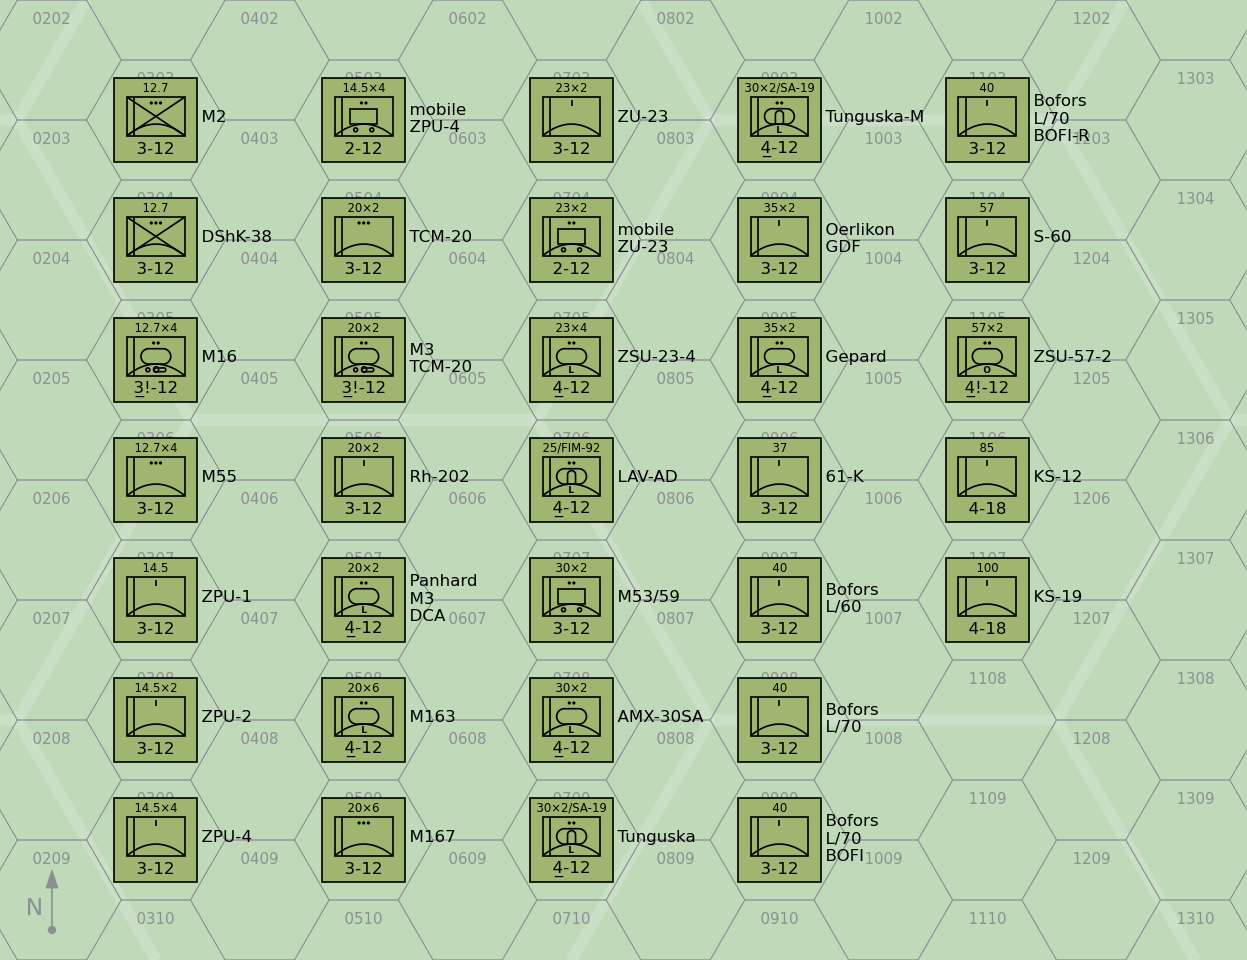
\includegraphics[height=0.4\linewidth]{figure-aaa.png}
    \caption{AAA Units}
    \label{figure:aaa-units}
\end{figure*}

\begin{figure*}
    \centering
    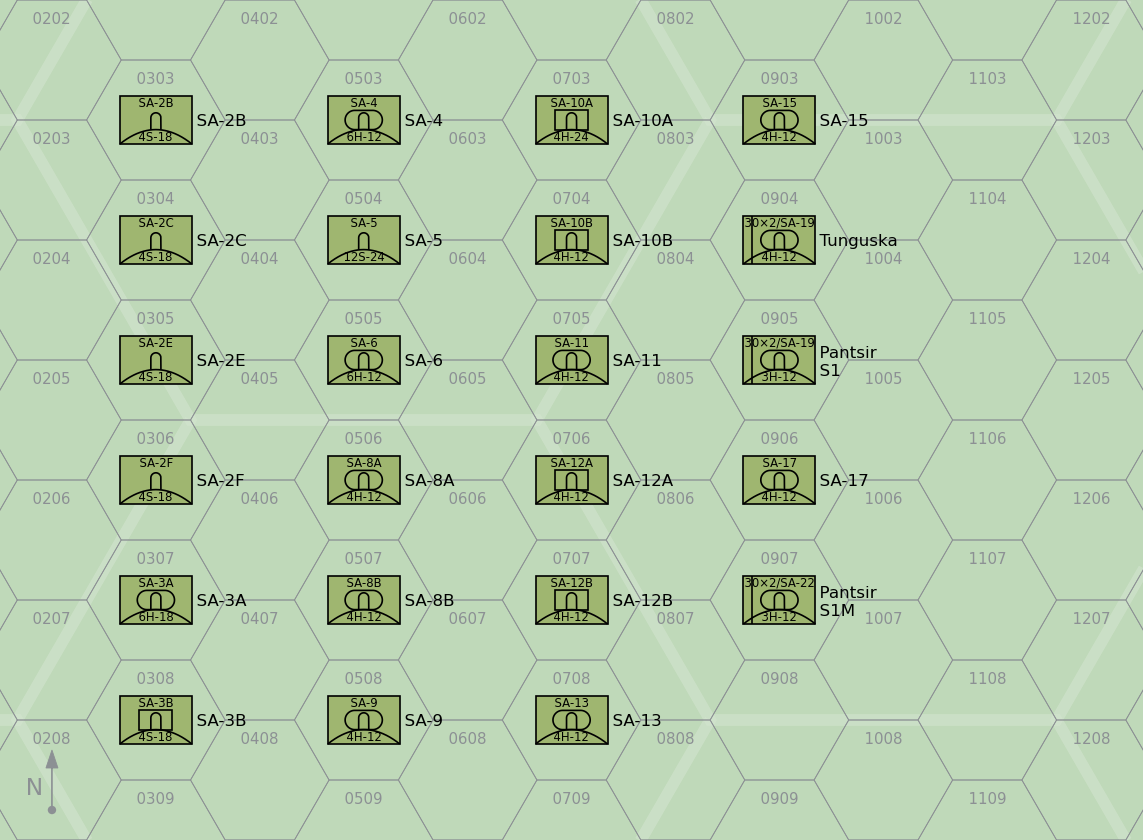
\includegraphics[height=0.4\linewidth]{figure-sam-launcher.png}
    \caption{SAM Launcher Units}
    \label{figure:sam-launcher-units}
\end{figure*}


\subsection{CCUs}

CCUs are air-defense command and control units. The generic CCU units are:
\begin{itemize}
    \item \emph{mobile CCU}
    \item \emph{armored CCU}
\end{itemize}

Mobile CCUs include the 9S737 Ranzhir.

Armored CCUs include the 9S80 PPRU-1.

\subsection{EWRs}

EWRs are air-defense early-warning radars. The generic EWR units are:
\begin{itemize}
    \item \emph{towed EWR-A}
    \item \emph{mobile EWR-A}
\end{itemize}

\subsection{FCRs}

FCRs are air-defense fire-control radars for towed AAA. The generic FCR units are:
\begin{itemize}
    \item \emph{towed FCR-A/B/C/D}
    \item \emph{mobile FCR-A/B/C/D}
\end{itemize}


\begin{table*}
    \caption{Generic Units}
    \centering
    \small
    \input{table-generic-units.tex}
    \label{table:generic-units}
\end{table*}

\twocolumn[\section{AAA Units}]

Table \ref{table:aaa-units} summarizes the properties of the AAA units. Soft and hard defense strengths are suffixed with S and H, respectively. The sighting range is given in hexes.

Figure \ref{figure:aaa-units} shows the graphical representation of the AAA units. Again, the representation uses NATO symbols.

\begin{table*}
    \caption{AAA Units}
    \centering
    \small
    \begin{tabularx}{\linewidth}{Lcclccc@{~}c@{~}cc@{~}c@{~}cccl}
\toprule
\\

            &
            &
            &
            &
            &
            &
            \multicolumn{3}{c}{Range}   &
            \multicolumn{3}{c}{Hit}     &
            &
            &
            \\
        

            \cmidrule(lr){7-9}
            \cmidrule(lr){10-12}
        

            Name&
            \multirow[b]{-3}{*}{\vertical{\begin{tabular}{@{}l@{}}Defense\\Strength\end{tabular}}}&
            \multirow[b]{-3}{*}{\vertical{\begin{tabular}{@{}l@{}}Sighting\\Range\end{tabular}}}&
            \multirow[b]{-3}{*}{\vertical{Gun}}       &
            \multirow[b]{-3}{*}{\vertical{Class}}       &
            \multirow[b]{-3}{*}{\vertical{Altitude}}    &
            S&M&L&       
            S&M&L&
            \multirow[b]{-3}{*}{\vertical{\begin{tabular}{@{}l@{}}Damage\\Rating\end{tabular}}}     &
            \multirow[b]{-3}{*}{\vertical{FCR}}&
            \multirow[b]{-3}{*}{\vertical{SAM}}\\
        
\midrule
\addlinespace
DShK-38&\wbox[l]{0H}{3S}&\wbox{00}{12}&12.7 mm&L&\wbox{00}{5}&\wbox{00}{2}&\wbox{00}{3}&\wbox{00}{4}&\wbox{00}{3}&\wbox{00}{2}&\wbox{00}{1}&\wbox{0}{1}&---&---\\
M2&\wbox[l]{0H}{3S}&\wbox{00}{12}&12.7 mm&L&\wbox{00}{5}&\wbox{00}{2}&\wbox{00}{3}&\wbox{00}{4}&\wbox{00}{3}&\wbox{00}{2}&\wbox{00}{1}&\wbox{0}{1}&---&---\\
M16&\wbox[l]{0H}{4H}&\wbox{00}{12}&\binarymultiply{12.7 mm}{4}&L&\wbox{00}{5}&\wbox{00}{2}&\wbox{00}{3}&\wbox{00}{4}&\wbox{00}{4}&\wbox{00}{3}&\wbox{00}{2}&\wbox{0}{2}&---&---\\
\addlinespace
M55&\wbox[l]{0H}{3S}&\wbox{00}{12}&\binarymultiply{12.7 mm}{4}&L&\wbox{00}{5}&\wbox{00}{2}&\wbox{00}{3}&\wbox{00}{4}&\wbox{00}{4}&\wbox{00}{3}&\wbox{00}{2}&\wbox{0}{2}&---&---\\
mobile M55&\wbox[l]{0H}{2S}&\wbox{00}{12}&\binarymultiply{12.7 mm}{4}&L&\wbox{00}{5}&\wbox{00}{2}&\wbox{00}{3}&\wbox{00}{4}&\wbox{00}{4}&\wbox{00}{3}&\wbox{00}{2}&\wbox{0}{2}&---&---\\
ZPU-1&\wbox[l]{0H}{3S}&\wbox{00}{12}&14.5 mm&L&\wbox{00}{6}&\wbox{00}{2}&\wbox{00}{3}&\wbox{00}{4}&\wbox{00}{3}&\wbox{00}{2}&\wbox{00}{1}&\wbox{0}{1}&---&---\\
\addlinespace
ZPU-2&\wbox[l]{0H}{3S}&\wbox{00}{12}&\binarymultiply{14.5 mm}{2}&L&\wbox{00}{6}&\wbox{00}{2}&\wbox{00}{3}&\wbox{00}{5}&\wbox{00}{4}&\wbox{00}{3}&\wbox{00}{1}&\wbox{0}{3}&---&---\\
ZPU-4&\wbox[l]{0H}{3S}&\wbox{00}{12}&\binarymultiply{14.5 mm}{4}&L&\wbox{00}{6}&\wbox{00}{2}&\wbox{00}{3}&\wbox{00}{5}&\wbox{00}{5}&\wbox{00}{4}&\wbox{00}{3}&\wbox{0}{2}&---&---\\
mobile ZPU-4&\wbox[l]{0H}{2S}&\wbox{00}{12}&\binarymultiply{14.5 mm}{4}&L&\wbox{00}{6}&\wbox{00}{2}&\wbox{00}{3}&\wbox{00}{5}&\wbox{00}{5}&\wbox{00}{4}&\wbox{00}{3}&\wbox{0}{2}&---&---\\
\addlinespace
Rh-202&\wbox[l]{0H}{3S}&\wbox{00}{12}&\binarymultiply{20 mm}{2}&L&\wbox{00}{8}&\wbox{00}{2}&\wbox{00}{4}&\wbox{00}{6}&\wbox{00}{3}&\wbox{00}{2}&\wbox{00}{1}&\wbox{0}{3}&---&---\\
Panhard M3 DCA&\wbox[l]{0H}{4H}&\wbox{00}{12}&\binarymultiply{20 mm}{2}&L&\wbox{00}{8}&\wbox{00}{2}&\wbox{00}{4}&\wbox{00}{6}&\wbox{00}{3}&\wbox{00}{3}&\wbox{00}{2}&\wbox{0}{2}&---&---\\
M163&\wbox[l]{0H}{4H}&\wbox{00}{12}&\binarymultiply{20 mm}{6}&L&\wbox{00}{8}&\wbox{00}{2}&\wbox{00}{4}&\wbox{00}{6}&\wbox{00}{6}&\wbox{00}{5}&\wbox{00}{4}&\wbox{0}{3}&R/HF&---\\
\addlinespace
M167&\wbox[l]{0H}{3H}&\wbox{00}{12}&\binarymultiply{20 mm}{6}&L&\wbox{00}{8}&\wbox{00}{2}&\wbox{00}{4}&\wbox{00}{6}&\wbox{00}{6}&\wbox{00}{5}&\wbox{00}{4}&\wbox{0}{3}&R/HF&---\\
ZU-23&\wbox[l]{0H}{3S}&\wbox{00}{12}&\binarymultiply{23 mm}{2}&L&\wbox{00}{9}&\wbox{00}{2}&\wbox{00}{5}&\wbox{00}{8}&\wbox{00}{4}&\wbox{00}{3}&\wbox{00}{2}&\wbox{0}{2}&---&---\\
mobile ZU-23&\wbox[l]{0H}{2S}&\wbox{00}{12}&\binarymultiply{23 mm}{2}&L&\wbox{00}{9}&\wbox{00}{2}&\wbox{00}{5}&\wbox{00}{8}&\wbox{00}{4}&\wbox{00}{3}&\wbox{00}{2}&\wbox{0}{2}&---&---\\
\addlinespace
ZSU-23-4&\wbox[l]{0H}{4H}&\wbox{00}{12}&\binarymultiply{23 mm}{4}&L&\wbox{00}{9}&\wbox{00}{2}&\wbox{00}{5}&\wbox{00}{8}&\wbox{00}{5}&\wbox{00}{4}&\wbox{00}{3}&\wbox{0}{3}&W/VF&---\\
AMX-30 DCA&\wbox[l]{0H}{4H}&\wbox{00}{12}&\binarymultiply{30 mm}{2}&L&\wbox{00}{10}&\wbox{00}{3}&\wbox{00}{6}&\wbox{00}{9}&\wbox{00}{5}&\wbox{00}{4}&\wbox{00}{3}&\wbox{0}{4}&W/VF&---\\
Tunguska&\wbox[l]{0H}{4H}&\wbox{00}{12}&\binarymultiply{30 mm}{2}&L&\wbox{00}{11}&\wbox{00}{4}&\wbox{00}{7}&\wbox{00}{9}&\wbox{00}{5}&\wbox{00}{4}&\wbox{00}{3}&\wbox{0}{4}&W/VF&SA-19\\
\addlinespace
Pantsir S1&\wbox[l]{0H}{3H}&\wbox{00}{12}&\binarymultiply{30 mm}{2}&L&\wbox{00}{11}&\wbox{00}{4}&\wbox{00}{7}&\wbox{00}{9}&\wbox{00}{5}&\wbox{00}{4}&\wbox{00}{3}&\wbox{0}{4}&W/VF&SA-19\\
Pantsir S1M&\wbox[l]{0H}{3H}&\wbox{00}{12}&\binarymultiply{30 mm}{2}&L&\wbox{00}{11}&\wbox{00}{4}&\wbox{00}{7}&\wbox{00}{9}&\wbox{00}{5}&\wbox{00}{4}&\wbox{00}{3}&\wbox{0}{4}&W/VF&SA-22\\
Oerlikon GDF&\wbox[l]{0H}{3S}&\wbox{00}{12}&\binarymultiply{35 mm}{2}&L&\wbox{00}{12}&\wbox{00}{4}&\wbox{00}{8}&\wbox{00}{10}&\wbox{00}{5}&\wbox{00}{4}&\wbox{00}{3}&\wbox{0}{4}&---&---\\
\addlinespace
Gepard&\wbox[l]{0H}{4H}&\wbox{00}{12}&\binarymultiply{35 mm}{2}&M&\wbox{00}{12}&\wbox{00}{4}&\wbox{00}{8}&\wbox{00}{12}&\wbox{00}{5}&\wbox{00}{4}&\wbox{00}{3}&\wbox{0}{5}&W/VF&---\\
M-38&\wbox[l]{0H}{3S}&\wbox{00}{12}&37 mm&M&\wbox{00}{12}&\wbox{00}{4}&\wbox{00}{8}&\wbox{00}{11}&\wbox{00}{3}&\wbox{00}{2}&\wbox{00}{1}&\wbox{0}{4}&---&---\\
Bofors L60&\wbox[l]{0H}{3S}&\wbox{00}{12}&40 mm&M&\wbox{00}{15}&\wbox{00}{4}&\wbox{00}{8}&\wbox{00}{12}&\wbox{00}{2}&\wbox{00}{2}&\wbox{00}{1}&\wbox{0}{4}&---&---\\
\addlinespace
Bofors L70&\wbox[l]{0H}{3S}&\wbox{00}{12}&40 mm&M&\wbox{00}{15}&\wbox{00}{4}&\wbox{00}{8}&\wbox{00}{12}&\wbox{00}{3}&\wbox{00}{3}&\wbox{00}{2}&\wbox{0}{4}&---&---\\
Bofors L70 BOFI-R&\wbox[l]{0H}{3S}&\wbox{00}{12}&40 mm&M&\wbox{00}{15}&\wbox{00}{4}&\wbox{00}{8}&\wbox{00}{12}&\wbox{00}{4}&\wbox{00}{4}&\wbox{00}{3}&\wbox{0}{4}&W/VF&---\\
M42&\wbox[l]{0H}{4H}&\wbox{00}{12}&\binarymultiply{40 mm}{2}&M&\wbox{00}{13}&\wbox{00}{4}&\wbox{00}{6}&\wbox{00}{11}&\wbox{00}{3}&\wbox{00}{2}&\wbox{00}{2}&\wbox{0}{5}&---&---\\
\addlinespace
S-60&\wbox[l]{0H}{3S}&\wbox{00}{12}&57 mm&M&\wbox{00}{18}&\wbox{00}{5}&\wbox{00}{10}&\wbox{00}{15}&\wbox{00}{1}&\wbox{00}{1}&\wbox{00}{0}&\wbox{0}{5}&---&---\\
ZSU-57-2&\wbox[l]{0H}{4H}&\wbox{00}{12}&\binarymultiply{57 mm}{2}&M&\wbox{00}{18}&\wbox{00}{5}&\wbox{00}{10}&\wbox{00}{15}&\wbox{00}{2}&\wbox{00}{1}&\wbox{00}{1}&\wbox{0}{5}&---&---\\
KS-12&\wbox[l]{0H}{4H}&\wbox{00}{18}&85 mm&H&\wbox{00}{27}&\wbox{00}{6}&\wbox{00}{12}&\wbox{00}{18}&\wbox{00}{2}&\wbox{00}{1}&\wbox{00}{0}&\wbox{0}{6}&---&---\\
\addlinespace
KS-19&\wbox[l]{0H}{4H}&\wbox{00}{18}&100 mm&H&\wbox{00}{39}&\wbox{00}{7}&\wbox{00}{14}&\wbox{00}{21}&\wbox{00}{2}&\wbox{00}{1}&\wbox{00}{0}&\wbox{0}{6}&---&---\\
\addlinespace
\bottomrule
\end{tabularx}

    \label{table:aaa-units}
\end{table*}

\twocolumn[\section{SAM Launcher Units}]


Table \ref{table:sam-launcher-units} summarizes the properties of the AAA units. Soft and hard defense strengths are suffixed with S and H, respectively. The sighting range is given in hexes.

Figure \ref{figure:sam-launcher-units} shows the graphical representation of the AAA units. Again, the representation uses NATO symbols.


\begin{table*}
    \caption{SAM Launcher Units}
    \centering
    \small
    \begin{tabularx}{\linewidth}{Lcccclcccccccccccl}
\toprule

            &
            &
            &
            &
            &
            &
            \multicolumn{3}{c}{EWR}         &
            \multicolumn{2}{c}{TTR}         &
            &
            \multicolumn{2}{c}{Missiles}    &
            &
            \multicolumn{2}{c}{Lock-On}     &
            \\
        

            \cmidrule(lr){7-9}
            \cmidrule(lr){10-11}
            \cmidrule(lr){13-14}
            \cmidrule(lr){16-17}
        

            Name&
            \vertical{Echelon}      &
            \vertical{\begin{tabular}{@{}l@{}}Defense\\Strength\end{tabular}}&
            \vertical{\begin{tabular}{@{}l@{}}Sighting\\Range\end{tabular}}&
            \vertical{\begin{tabular}{@{}l@{}}VPs\\K/2D/D\end{tabular}}&
            \multicolumn{1}{c}{\multirow[b]{-3}{*}{\vertical{SAM}}}&
            \vertical{Frequency}    &
            \vertical{Range}        &
            \vertical{MTI}          &
            \vertical{Frequency}    &
            \vertical{Range}        &
            \vertical{\begin{tabular}{@{}l@{}}Multi-Target\\Capability\end{tabular}}&
            \vertical{Ready}        &
            \vertical{Volley}       &
            \vertical{\begin{tabular}{@{}l@{}}Quick\\Reaction\end{tabular}}&
            \vertical{Radar}        &
            \vertical{Optical}      &
            \vertical{Gun}          \\
            
\midrule
SA-2B &\wbox[l]{Section}{Battery}&\wbox[l]{0}{4}&\wbox{00}{18}&\wbox{0/0/0}{8/5/3}&SA-2B&LF&\wbox{000}{30}&---&LF&\wbox{00}{20}&---&\wbox{00}{6}&\wbox{00}{2}&---&6&---&---\\
SA-2C &\wbox[l]{Section}{Battery}&\wbox[l]{0}{4}&\wbox{00}{18}&\wbox{0/0/0}{8/5/3}&SA-2C&LF&\wbox{000}{30}&---&MF&\wbox{00}{20}&---&\wbox{00}{6}&\wbox{00}{2}&---&6&---&---\\
SA-2E &\wbox[l]{Section}{Battery}&\wbox[l]{0}{4}&\wbox{00}{18}&\wbox{0/0/0}{8/5/3}&SA-2E&LF&\wbox{000}{30}&---&MF&\wbox{00}{20}&---&\wbox{00}{6}&\wbox{00}{2}&---&6&---&---\\
SA-2F &\wbox[l]{Section}{Battery}&\wbox[l]{0}{4}&\wbox{00}{18}&\wbox{0/0/0}{8/5/3}&SA-2F&LF&\wbox{000}{30}&---&LF&\wbox{00}{20}&---&\wbox{00}{6}&\wbox{00}{2}&---&6&6&---\\
SA-3A &\wbox[l]{Section}{Battery}&\wbox[l]{0}{4}&\wbox{00}{18}&\wbox{0/0/0}{10/7/4}&SA-3B&LF&\wbox{000}{30}&---&HF&\wbox{00}{10}&---&\wbox{00}{16}&\wbox{00}{2}&---&6&6&---\\
Mobile SA-3A &\wbox[l]{Section}{Battery}&\wbox[l]{0}{4}&\wbox{00}{18}&\wbox{0/0/0}{12/8/4}&SA-3B&LF&\wbox{000}{30}&---&HF&\wbox{00}{10}&---&\wbox{00}{8}&\wbox{00}{2}&---&6&6&---\\
SA-4 &\wbox[l]{Section}{Battery}&\wbox[l]{0}{\underline{3}}&\wbox{00}{12}&\wbox{0/0/0}{10/6/3}&SA-4&---&\wbox{000}{---}&---&HF&\wbox{00}{30}&---&\wbox{00}{6}&\wbox{00}{2}&---&7&---&---\\
SA-6A &\wbox[l]{Section}{Battery}&\wbox[l]{0}{\underline{6}}&\wbox{00}{12}&\wbox{0/0/0}{11/7/4}&SA-6A&MF&\wbox{000}{24}&---&HF&\wbox{00}{18}&---&\wbox{00}{12}&\wbox{00}{2}&---&7&6&---\\
SA-6B &\wbox[l]{Section}{Battery}&\wbox[l]{0}{\underline{6}}&\wbox{00}{12}&\wbox{0/0/0}{12/8/4}&SA-6B&MF&\wbox{000}{24}&---&HF&\wbox{00}{18}&---&\wbox{00}{12}&\wbox{00}{2}&---&7&6&---\\
SA-7A &\wbox[l]{Section}{Section}&\wbox[l]{0}{5}&\wbox{00}{6}&\wbox{0/0/0}{10/6/3}&SA-7A&---&\wbox{000}{---}&---&---&\wbox{00}{---}&---&\wbox{00}{1}&\wbox{00}{1}&Y&---&7&---\\
SA-7B &\wbox[l]{Section}{Section}&\wbox[l]{0}{\underline{5}}&\wbox{00}{6}&\wbox{0/0/0}{0/0/0}&SA-7B&MF&\wbox{000}{24}&---&HF&\wbox{00}{18}&---&\wbox{00}{12}&\wbox{00}{3}&---&7&6&---\\
SA-8B &\wbox[l]{Section}{Squad}&\wbox[l]{0}{\underline{4}}&\wbox{00}{12}&\wbox{0/0/0}{0/0/0}&SA-8B&HF&\wbox{000}{10}&---&VF&\wbox{00}{6}&2&\wbox{00}{6}&\wbox{00}{2}&Y&8&7&---\\
SA-9 &\wbox[l]{Section}{Squad}&\wbox[l]{0}{\underline{4}}&\wbox{00}{12}&\wbox{0/0/0}{0/0/0}&SA-9&---&\wbox{000}{---}&---&---&\wbox{00}{---}&2&\wbox{00}{4}&\wbox{00}{2}&---&---&7&---\\
SA-11 &\wbox[l]{Section}{Squad}&\wbox[l]{0}{\underline{4}}&\wbox{00}{12}&\wbox{0/0/0}{0/0/0}&SA-11&HF&\wbox{000}{50}&---&HF&\wbox{00}{18}&2&\wbox{00}{4}&\wbox{00}{2}&---&8&7&---\\
SA-13 &\wbox[l]{Section}{Squad}&\wbox[l]{0}{\underline{4}}&\wbox{00}{12}&\wbox{0/0/0}{0/0/0}&SA-13&---&\wbox{000}{---}&---&---&\wbox{00}{---}&2&\wbox{00}{4}&\wbox{00}{2}&Y&---&8&---\\
SA-14 &\wbox[l]{Section}{Section}&\wbox[l]{0}{\underline{5}}&\wbox{00}{6}&\wbox{0/0/0}{0/0/0}&SA-14&MF&\wbox{000}{24}&---&HF&\wbox{00}{18}&---&\wbox{00}{12}&\wbox{00}{3}&---&7&6&---\\
SA-15 &\wbox[l]{Section}{Squad}&\wbox[l]{0}{\underline{4}}&\wbox{00}{12}&\wbox{0/0/0}{0/0/0}&SA-15&HF&\wbox{000}{30}&Y&MW&\wbox{00}{20}&2&\wbox{00}{8}&\wbox{00}{2}&Y&9&8&---\\
\addlinespace
\bottomrule
\end{tabularx}

    \label{table:sam-launcher-units}
\end{table*}

\end{document}